\documentclass{beamer}
\usepackage{graphicx,url}

\usepackage{amsmath}
\usepackage{amssymb}
\usepackage{xkeyval}

\usepackage{../macros/mytikz}
\usepgflibrary{shapes}
\usepackage{stmaryrd}

\usepackage{../macros/basics}
\usepackage{../macros/basics-slides}
%\usepackage{../macros/mmt_listings}
\usepackage{../macros/twelf-math}

\usepackage{macros}
\usepackage{../macros}

\newcommand{\lf}{\mathit{LF}}
\newcommand{\kity}{\mathit{type}}


\renewcommand{\emph}[1]{\alert{#1}}

%\setbeamertemplate{headline}{\small\hfill\insertsection \hfill\hbox{}}

\begin{document}

\title{Knowledge Representation and Processing}
\author{Florian Rabe (for a course given with Michael Kohlhase)}
\institute{Computer Science, University Erlangen-N\"urnberg, Germany}
\date{Summer 2020}
\begin{frame}
    \titlepage
\end{frame}

\section{Administrative Information}

\begin{frame}\frametitle{Format}
\begin{blockitems}{Zoom}
\item lectures and exercises via zoom
\item participants muted by default for simplicity
\item interaction strongly encouraged
 \lec{We don't want to lecture ---}
 \lec{we want to have a conversation during which you learn}
\item let's try out zoom
 \begin{itemize}
 \item use reactions to say yes no, ask for break etc.
 \item feel free to annotate my slides
 \item talk in the chat
 \end{itemize}
\end{blockitems}

\begin{blockitems}{Recordings}
\item maybe prerecorded video lectures or recorded zoom meeting
\item to be decided along the way
\end{blockitems}
\end{frame}


\begin{frame}\frametitle{Background}
\begin{blockitems}{Instructors}
\item Prof. Dr. Michael Kohlhase \lec{Professor of Knowledge Representation and Processing}
\item PD Dr. Florian Rabe \lec{same research group}
\end{blockitems}

\begin{blockitems}{Course}
\item This course is given for the first time
\item Always a little bit of an experiment
  \lec{cutting edge vs. unpolished}
\item Could become signature course of our research group \lec{same name!}
\end{blockitems}
\end{frame}

\begin{frame}\frametitle{Prerequisites}
\begin{blockitems}{Required}
\item basic knowledge about formal languages, context-free grammars
 \lec{but we'll do a quick revision here}
\end{blockitems}

\begin{blockitems}{Helpful}
\item Algorithms and Data Structures
 \lec{mostly as a contrast to this lecture}
\item Basic logic
 \lec{we'll revise it slightly differently here}
\item all other courses
 \lec{as examples of how knowledge pervades all of CS}
\end{blockitems}

\begin{blockitems}{General}
\item Curiosity \lec{this course is a bit unusual}
\item Interest in big picture \lec{this course touches on lots of things from all over CS}
\end{blockitems}
\end{frame}

\begin{frame}\frametitle{Examination and Grading}
\begin{blockitems}{Suggestion}
\item grade determined by single exam
\item written or oral \lec{depends on number of students}
\item some acknowledgment for practical exercises
\end{blockitems}
\lec{to be finalized next week}

\begin{blockitems}{Exam-relevant}
\item anything mentioned in notes
\item anything discussed in lectures
\end{blockitems}
\lec{neither is a superset of the other!}
\end{frame}

\begin{frame}\frametitle{Materials and Exam-Relevance}
\begin{blockitems}{Textbook}
\item does not exist
\item normal for research-near specialization courses
\end{blockitems}

\begin{blockitems}{Notes}
\item textbook-style but not as comprehensive
\item developed along the way
\end{blockitems}

\begin{blockitems}{Slides}
\item not comprehensive
\item used as visual aid, conversation starters
\end{blockitems}
\end{frame}

\begin{frame}\frametitle{Communication}
\begin{blockitems}{Open for questions}
\item open door policy in our offices
  \glec{if the lockdown ever ends}
\item always room for questions during lectures
\item for personal questions, contact me during/after lecture or by email
\item forum at \url{https://fsi.cs.fau.de/forum/154-Wissensrepraesentation-und-Verarbeitung}
\end{blockitems}

\begin{blockitems}{Materials}
\item official notes and slides as pdf: \url{https://kwarc.info/teaching/WuV/}
 \lec{will be updated from time to time}
\item watch me prepare the materials: \url{https://github.com/florian-rabe/Teaching/tree/master/WuV}
 \lec{pull requests and issues welcome}
\end{blockitems}
\end{frame}

\begin{frame}\frametitle{Exercises}
\begin{blockitems}{Learning Goals}
\item Get acquainted with state of the art of practice
\item Try out real tools
\end{blockitems}

\begin{blockitems}{Homeworks}
\item one major project as running example
\item homeworks building on each other
\end{blockitems}
\lec{build one large knowledge-based system}
\lec{details on later slides}
\end{frame}

\section{Overview and Essential Concepts}

\begin{frame}\frametitle{Representation and Processing}
Common pairs of concepts:
\begin{center}
\begin{tabular}{l|l}
Representation & Processing \\
\hline
Static & Dynamic \\
Situation & Change \\
Be & Become \\
Data Structures & Algorithms \\
Set & Function \\
State & Transition \\
Space & Time
\end{tabular}
\end{center}
\end{frame}

\begin{frame}\frametitle{Data and Knowledge}
$2\times 2$ key concepts
\begin{center}
\begin{tabular}{l|l}
Syntax & Data \\
\hline
Semantics & Knowledge
\end{tabular}
\end{center}

\begin{itemize}
\item Data: any object that can be stored in a computer\\
 Example: $((49.5739143, 11.0264941), "2020-04-21T16:15:00CEST")$
\item Syntax: a system of rules that describes which data is \textbf{well-formed}\\
 Example: ``a pair of (a pair of two IEEE double precision floating point numbers) and a string encoding of a time stamp''
\item Semantics: system of rules that determines the meaning of well-formed data
\item Knowledge: combination of some data with its syntax and semantics
\end{itemize}
\end{frame}

\begin{frame}\frametitle{Knowledge is Elusive}
Representation of key concepts 
\begin{itemize}
 \item Data: using primitive objects
  \lec{implemented as bits, bytes, strings, records, arrays, \ldots}
 \item Syntax: (context-free) grammars, (context-sensitive) type systems
  \lec{implemeted as inductive data structures}
 \item Semantics: functions for evaluation, interpretation, of well-formed data
  \lec{implemented as recursive algorithms on the syntax}
 \item Knowledge: elusive
  \lec{emerges from applying and interacting with the semantics}
\end{itemize}
\end{frame}

\begin{frame}\frametitle{Semantics as Translation}
\begin{itemize}
\item Knowledge can be captured by a higher layer of syntax
\item Then semantics is translation into syntax
\end{itemize}

\begin{center}
\begin{tabular}{l|l|l}
Data syntax & Semantics function & Knowledge syntax \\
\hline
SPARQL query & evaluation & result set \\
SQL query & evaluation & result table \\
program & compiler & binary code \\
program expression & interpreter & result value \\ 
logical formula & interpretation in a model & mathematical object \\
HTML document & rendering & graphics context
\end{tabular}
\end{center}
\end{frame}

\begin{frame}\frametitle{Heterogeneity of Data and Knowledge}
\begin{itemize}
\item Capturing knowledge is difficult
\item Many different approaches to semantics
 \begin{itemize}
  \item fundamental formal and methodological differences
  \item often captured in different fields, conferences, courses, languages, tools
 \end{itemize}
\item Data formats equally heterogeneous
 \begin{itemize}
 \item ontologies
 \item programs
 \item logical proofs
 \item databases
 \item documents
 \end{itemize}
\end{itemize}
\end{frame}

\begin{frame}\frametitle{Challenges of Heterogeneity}
\begin{blockitems}{Challenges}
\item collaboration across communities
\item translation across languages
\item conversion between data formats
\item interoperability across tools
\end{blockitems}

\begin{blockitems}{Sources of problems}
\item interoperability across formats/tools major source of
 \begin{itemize}
 \item complexity
 \item bugs
 \end{itemize}
\item friction in project team due to differing preferences, expertise
\item difficult choice between languages/tools with competing advantages
\begin{itemize}
 \item reverting choices difficult, costly
 \item maintaining legacy choices increases complexity
\end{itemize}
\end{blockitems}
\end{frame}

\begin{frame}\frametitle{Aspects of Knowledge}
\begin{itemize}
\item Tetrapod model of knowledge
  \lec{active research by our group}
\item classifies approaches to knowledge into five aspects
\end{itemize}

\begin{center}
\begin{tabular}{lll}
Aspect & KRLs (examples) & KPTs (examples) \\
\hline
ontologization & ontology languages (OWL), description logics (ALC) & reasoners, SPARQL engines (Virtuoso) \\
concretization & relational databases (SQL, JSON) & databases (MySQL, MongoDb) \\
computation & programming languages (C) & interpreters, compilers (gcc) \\
deduction & logics (HOL) & theorem provers (Isabelle) \\
narration & document languages (HTML, LaTeX) & editors, viewers
\end{tabular}
\end{center}
\end{frame}

\begin{frame}\frametitle{Relations between the Aspects}
Ontology is distinguished: capture the knowledge that the other four aspects share

\begin{center}
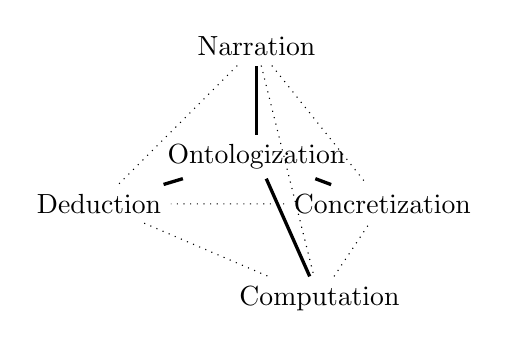
\begin{tikzpicture}[scale=4]
  \node (center) at (0,.15) {Ontologization};
  \node (left) at (.2,-.3) {Computation};
  \node (right) at (.4,0) {Concretization};
  \node (back) at (-.5,0) {Deduction};
  \node (up) at (0,.5) {Narration};

  \draw[very thick] (center) -- (left);
  \draw[very thick] (center) -- (right);
  \draw[very thick] (center) -- (back);
  \draw[very thick] (center) -- (up);
  \draw[dotted] (left) -- (right) -- (back) -- (left);
  \draw[dotted] (up) -- (left);
  \draw[dotted] (up) -- (right);
  \draw[dotted] (up) -- (back);
\end{tikzpicture}
\end{center}
\end{frame}

\begin{frame}\frametitle{Complementary Advantages of the Aspects}
\begin{center}
\footnotesize
\begin{tabular}{|l|llp{2.1cm}l|}\hline
Aspect & objects & \multicolumn{3}{c|}{characteristic} \\
       &         & advantage & joint advantage of the other aspects & application \\\hline
ded. & formal proofs & correctness & ease of use & verification \\
comp. & programs & efficiency & well-definedness & execution\\
concr. & concrete objects & tangibility & abstraction & storage/retrieval\\
narr. & texts & flexibility & formal semantics & human understanding\\\hline
\end{tabular}
\medskip

\begin{tabular}{|l|l|}\hline
Aspect pair & characteristic advantage \\\hline
ded./comp.  & rich meta-theory \\
narr./conc. & simple languages \\\hline
ded./narr.  & theorems and proofs \\
comp./conc. & normalization \\\hline
ded./conc.  & decidable well-definedness \\
comp./narr. & Turing completeness \\\hline
\end{tabular}
\end{center}
\end{frame}

\begin{frame}\frametitle{Structure of the Course}
\begin{blockitems}{Aspect-independent parts}
\item general methods that are shared among the aspects
\item to be discussed as they come up
\end{blockitems}

\begin{blockitems}{Aspects-specific parts}
\item one part (about 2 weeks) for each aspect
\item high-level overview of state of the art
\item focus on comparison/evaluation of the aspect-specific results
\end{blockitems}
\end{frame}

\begin{frame}\frametitle{Structure of the Exercises}
\begin{blockitems}{One major project}
\item representative for a project that a CS graduate might be put in charge of
\item challenging heterogeneous data and knowledge
\item requires integrating/combining different languages, tools
\end{blockitems}
\lec{unique opportunity in this course because knowledge is everywhere}

\begin{blockitems}{Concrete project}
\item develop a univis-style system for a university
\item lots of heterogeneous knowledge
 \begin{itemize}
 \item course and program descriptions
 \item legal texts
 \item websites
 \item grade tables
 \item transcript generation code
 \end{itemize} 
\item build a completely functional system applying the lessons of the course
\end{blockitems}
\end{frame}

\section{Ontological Knowledge}

\begin{frame}\frametitle{Components of an Ontology}
8 main declarations
\begin{itemize}
 \item \textbf{individual} --- concrete objects that exist in the real world, e.g., "Florian Rabe" or "WuV"
 \item \textbf{concept} --- abstract groups of individuals, e.g., "instructor" or "course"
 \item \textbf{relation} --- binary relations between two individuals, e.g., "teaches"
 \item \textbf{properties} --- binary relations between an individuals and a concrete value (a number, a date, etc.), e.g., "has-credits"
 \item \textbf{concept assertions} --- the statement that a particular individual is an instance of a particular concept
 \item \textbf{relation assertions} --- the statement that a particular relation holds about two individuals
 \item \textbf{property assertions} --- the statement that a particular individual has a particular value for a particular property
 \item \textbf{axioms} --- statements about relations between concepts, e.g., "instructor" $\sqsubseteq$ "person"
\end{itemize}
\end{frame}

\begin{frame}\frametitle{Divisions of an Ontology}
\begin{blockitems}{Abstract vs. concrete}
 \item TBox: concepts, relations, properties, axioms
  \lec{everything that does not use individuals}
 \item ABox: individuals and assertions
\end{blockitems}

\begin{blockitems}{Named vs. unnamed}
 \item Signature: individuals, concepts, relations, properties \lec{together called entities or resources}
 \item Theory: assertions, axioms
\end{blockitems}
\end{frame}

\begin{frame}\frametitle{Comparison of Terminology}
\begin{center}
\tiny
\begin{tabular}{l|llll|l}
 Here       & OWL      & Description logics & ER model & UML & semantics via logics\\
\hline
 individual & instance & individual & entity & object, instance & constant\\
 concept    & class    & concept &  entity-type & class & unary predicate\\
 relation   & object property & role & role & association & binary predicate \\
 property   & data property   & (not common) & attribute & field of base type & binary predicate\\
\end{tabular}
\medskip

\begin{tabular}{l|ll}
 domain & individual & concept \\
\hline
type theory, logic & constant, term & type \\
set theory  & element & set \\
database    & row & table \\
philosophy\footnote{as in \url{https://plato.stanford.edu/entries/object/}} & object & property \\
grammar & proper noun & common noun \\
\end{tabular}
\end{center}
\end{frame}

\begin{frame}\frametitle{Ontologies as Sets of Triples}
\begin{center}
\begin{tabular}{l|lll}
Assertion & \multicolumn{3}{c}{Triple} \\
          & Subject & Predicate & Object \\
\hline
concept assertion  & "Florian Rabe" & \texttt{is-a} & "instructor" \\
relation assertion & "Florian Rabe" & "teaches" & "WuV" \\
property assertion & "WuV" & "has credits" & 7.5 \\
\end{tabular}
\medskip

Efficient representation of ontologies using RDF and RDFS standardized special entities.
\end{center}
\end{frame}

\begin{frame}\frametitle{Special Entities}
RDF and RDFS define special entities for use in ontologies:
\begin{itemize}
 \item "rdfs:Resource": concept of which all individuals are an instance and thus of which every concept is a subconcept
 \item "rdf:type": relates an entity to its type:
  \begin{itemize}
   \item an individual to its concept (corresponding to \texttt{is-a} above)
   \item other entities to their special type (see below)
  \end{itemize}
 \item "rdfs:Class": special class for the type of classes
 \item "rdf:Property": special class for the type of properties
 \item "rdfs:subClassOf": a special relation that relates a subconcept to a superconcept
% \item "rdfs:subPropertyOf": a special relation that relates a relation to one that it implies
 \item "rdfs:domain": a special relation that relates a relation to the concepts of its subjects
 \item "rdfs:range": a special relation that relates a relation/property to the concept/type of its objects
\end{itemize}

Goal/effect: capture as many parts as possible as RDF triples.
\end{frame}

\begin{frame}\frametitle{Declarations as Triples using Special Entities}
\begin{center}
\begin{tabular}{l|lll}
Assertion & \multicolumn{3}{c}{Triple} \\
          & Subject & Predicate & Object \\
\hline
individual & individual & "rdf:type" & "rdfs:Resource" \\
concept  & concept & "rdf:type" & "rdf:Class" \\
relation & relation & "rdf:type" & "rdf:Property" \\
property & property & "rdf:type" & "rdf:Property" \\
concept assertion  & individual & "rdf:type" & concept \\
relation assertion & individual & relation & individual \\
property assertion & individual & property & value \\
\hline
\multicolumn{4}{l}{for special forms of axioms}\\
$c\sqsubseteq d$ & $c$ & "rdfs:subClassOf" & $d$ \\
%$r\sqsubseteq s$ & $r$ & "rdfs:subPropertyOf" & s \\
$\dom\,r\Equiv c$ & $r$ & "rdfs:domain" & $c$ \\
$\rng\, r\Equiv c$ & $r$ & "rdfs:range" & $c$ \\
\end{tabular}
\end{center}
\end{frame}

\begin{frame}\frametitle{An Example Ontology Language}
see syntax and semantics in the lecture notes
\end{frame}

\section{Representing Formal Languages}

\begin{frame}\frametitle{Example: Syntax of Arithmetic Language}
Syntax: represented as formal grammar

\begin{commgrammar}
\gcomment{Numbers}\\
\gprod{N}{0\bnfalt 1}{literals}\\
\galtprod{N+N}{sum}\\
\galtprod{N*N}{product}\\
\gcomment{Formulas}\\
\gprod{F}{N\doteq N}{equality}\\
\galtprod{N\leq N}{ordering by size}\\
\end{commgrammar}

Implementation as inductive data type
\end{frame}


\begin{frame}\frametitle{Example: Semantics of Arithmetic Language}
Semantics: represented as translation into known language
\medskip

Problem: Need to choose a known language first\\
Here: unary numbers represented as strings

Built-in data (strings and booleans):
\begin{commgrammar}
%\gcomment{Strings}\\
\gprod{S}{\epsilon}{empty}\\
\galtprod{(\texttt{Unicode)}}{characters}\\
%\gcomment{Booleans}\\
\gprod{B}{\cn{true}}{truth}\\
\galtprod{\cn{false}}{falsity}\\
\end{commgrammar}

Built-in operations to work on the data:
\begin{itemize}
\item concatenation of strings $S\bbc \cn{conc}(S,S)$
\item replacing all occurrences of $c$ in $S_1$ with $S_2$ $S\bbc \cn{replace}(S_1,c,S_2)$
\item equality test: $B\bbc S_1==S_2$
\item prefix test: $B\bbc \cn{startsWith}(S_1,S_2)$
\end{itemize}
\end{frame}

\begin{frame}\frametitle{Example: Semantics of Arithmetic Language}
\begin{blockitems}{Represented as function from syntax to semantics}
\item mutually recursive, inductive functions for each non-terminal symbol
\item compositional: recursive call on immediate subterms of argument
\end{blockitems}

For numbers $n$: semantics $\sem{n}$ is a string
\begin{itemize}
\item $\sem{0}=\epsilon$
\item $\sem{1}="|"$
\item $\sem{m+n}=\cn{conc}(\sem{m},\sem{n})$
\item $\sem{m*n}=\cn{replace}(\sem{m},"|",\sem{n})$
\end{itemize}
\medskip

For formulas $f$: semantics $\sem{f}$ is a boolean
\begin{itemize}
\item $\sem{m\doteq n}=\sem{m}==\sem{n}$
\item $\sem{m\leq n}=\cn{startsWith}(\sem{n},\sem{m})$
\end{itemize}
\end{frame}
\end{document}

%%% Local Variables:
%%% mode: latex
%%% TeX-master: t
%%% mode: visual-line
%%% fill-column: 5000
%%% End:

